\documentclass{article}
\usepackage{graphicx} % Required for inserting images
\usepackage[T2A]{fontenc}
\usepackage[utf8]{inputenc}
\usepackage[english,russian]{babel}
\usepackage[tbtags]{amsmath}
\usepackage{amsfonts,amssymb,mathrsfs,amscd}
\usepackage{graphicx}
\usepackage{subcaption}
\usepackage{comment}
\usepackage{ esint }
\usepackage{ amssymb }
\usepackage{ dsfont }
\usepackage{ stmaryrd }
\usepackage{ tipa }
\usepackage{placeins}
\usepackage{amsmath}
\usepackage{ upgreek }
\usepackage{adjustbox}





\title{Отчёт по задаче №3.28}
\author{Орлов Даниил Ильич}
\date{December 2024}
\begin{document}
	
	\maketitle
	
\section{Постановка Задачи:}
Необходимо найти решение данной задачи:

\begin{equation*}
	\left\{ \begin{aligned} 
		&\frac{\partial^2u}{\partial t^2} = \frac{\partial^2u}{\partial x^2} + 2\frac{\partial u}{\partial x} + u,\\
		&x = 0: u = sin^2(3t);\\
		&x = 1: \frac{\partial u}{\partial x} = \frac{t}{1 + t^2};\\
		&t = 0: u = \frac{\partial u}{\partial t} = 0.
	\end{aligned} \right.
\end{equation*}
	
Её будем решать следующим образом: 
	\begin{enumerate}
		\item Сначала возьмём равномерную сетку $\Omega = \{(x_m, t^n) = (mx, n\tau) | m\in\{0, ..., M\}, n\in\{0, ..., N\}\}.$
		\item Сначала подберём нужную схему.
		\item Поймём про порядок аппроксимации, желательно(даже необходимо, чтобы она была не ниже второго порядка).
		\item Выясним, является ли наша схема спектрально-устойчивой(будем добиваться её устойчивости).
		\item Посмотрим на решение и на график.
		\item Проведём нужные тесты.
	\end{enumerate}
	
\section{Схема:}
Предлагаю следующую схему, подобную схему "Крест":
\[
	\frac{u^{n + 1}_m - 2u^n_m + u^{n - 1}_m}{\tau^2} = \frac{u^n_{m + 1} - 2u^n_m + u^n_{m - 1}}{h^2} - \frac{u^n_{m + 1} - u^n_{m - 1}}{h} + u^n_m
\]

Поймём про её порядок, для этого разложим в ряд Тейлора $u^{n\pm 1}_{m\pm 1}$:
\[
	u^{n\pm 1}_{m\pm 1} = u^n_m \pm h\cdot\frac{\partial u}{\partial x} 
	\pm\tau\cdot\frac{\partial u}{\partial t} + \frac{h^2}{2!}\cdot\frac{\partial^2 u}{\partial x^2} + \frac{\tau^2}{2!}\cdot\frac{\partial^2 u}{\partial t^2} + h\cdot\tau\cdot\frac{\partial^2 u}{\partial xt} +  ...\text{ третьи производные }... + \underline O(\tau^4 + h^4)
\]

	Подставим в нашу схему и получим следующее:
\[
	\frac{\partial^2 u}{\partial t^2} = \frac{\partial^2 u}{\partial x^2} + 2\cdot\frac{\partial u}{\partial x} + u + \underline O(\tau^2 + h^2).
\]
	
Для спектральной устойчивости сделаем замену $u^n_m = u^n_m + \delta u^n_m$ и подставим:

\[
	\frac{\delta u^{n + 1}_m - 2\delta u^n_m + \delta u^{n - 1}_m}{\tau^2} = \frac{\delta u^n_{m + 1} - 2\delta u^n_m + \delta u^n_{m - 1}}{h^2} - \frac{\delta u^n_{m + 1} - \delta u^n_{m - 1} }{h} + \delta u^n_m.
\]
И сделаем замену: $\delta u^n_m = \lambda^n\cdot e^{im\phi}$
\[
	\frac{\lambda^2 - 2\lambda + 1}{\tau^2} = \frac{\lambda(e^{-i\phi} - 2 + e^{im\phi})}{h^2}.
\]
	Получаем:
\[
	\lambda^2 - 2(1 - \frac{2\tau^2 sin^2(\frac{\phi}{2})}{h^2})\lambda + 1 = 0.
\]
	$\forall \phi \in [0, 2\pi]$ заметим, что произведение корней по модулю $\lambda_1 \lambda_2 = 1$. Тогда, если у нас корни $\in \mathds{R}$, то тогда один корень точно  $ > 1 $. Следовательно нет устойчивости.
	Если у нас корни $\in \mathds{C}$, то тогда имеется спектральная устойчивость. Осталось понять условия для двух комплексных корней:
	нужно, чтобы дискриминант $D < 0$.
	
\[
	\frac{D}{4} = (2(1 - \frac{2\tau^2 sin^2(\frac{\phi}{2})}{h^2}))^2 - 1 = 
	4\frac{\tau^2sin^2(\frac{\phi}{2})(\frac{\tau^2sin^2(\frac{\phi}{2})}{h^2} - 1)}{h^2} < 0.
\]
Тогда это верно, если $\tau \leqslant h$.
	
	
\section{Решение:}

Вернёмся к нашей схеме:
\[
\frac{u^{n + 1}_m - 2u^n_m + u^{n - 1}_m}{\tau^2} = \frac{u^n_{m + 1} - 2u^n_m + u^n_{m - 1}}{h^2} - \frac{u^n_{m + 1} - u^n_{m - 1}}{h} + u^n_m
\]
Тогда из неё выразим слагаемое $u^{n + 1}_m$:
\[
	u^{n + 1}_m = 2u^n_m - u^{n + 1}_m + \frac{\tau^2(u^n_{m + 1} - 2u^n_m + u^n_{m - 1})}{h^2} - \frac{\tau^2(u^n_{m + 1} - u^n_{m - 1})}{h} + \tau^2u^n_m.
\]
Это общая формула для вычисления внутренних точек последующего слоя, для неё нужно знать значения точек на двух предыдущих слоёв. Может возникнуть, как считать нулевой слой и первый, но о них чуть позже. Разберёмся с граничными условиями.$\newline$
Для $x = 0: $ 
\[
	u^n_0 = sin^2(3t_n);
\]
	
Для $x = 1: $
\[
	\frac{\partial u}{\partial x} = \frac{t}{1 + t^2_n}.
\]
Приблизим нашу производную следующим образом: $\frac{\partial u}{\partial x} = \frac{u^n_M - u^n_{M-1}}{h}$.  Выведем нужную формулу: 
\[
	u^n_M = u^m_{N - 1} + \frac{ht_n}{1 + t^2_n}.
\]
В итоге мы получим все точки на новом слое. 
Разберёмся теперь с нулевым и первым слоем:
$\newline$
На нулевом слое все внутренние точки и граничные равны 0, значит весь нулевой слой - нулевой.
На первом слое сделаем следующее: для внутренних точек разложим в ряд Тейлора до второго порядка: $u^1_m = u^0_m + \tau\frac{\partial u}{\partial t}|_{t = 0} + \frac{\tau^2}{2}\frac{\partial^2u}{\partial t^2}$, все слагаемые равны нулю, следовательно все внутренние точки тоже равны нулю. Разберёмся с граничными:$\newline$
Для $x = 0: $
\[
	u^1_0 = sin^2(3\tau).
\]	
Для $x = 1: $
\[
	u^1_N = u^1_{N - 1} + \frac{\tau h}{1 + \tau^2}.
\] 
	
Вычислительные формулы написаны.

Посмотрим на графики: 
	\begin{figure}[h]
	\centering 
	\begin{minipage}{0.45\textwidth}
		\centering
		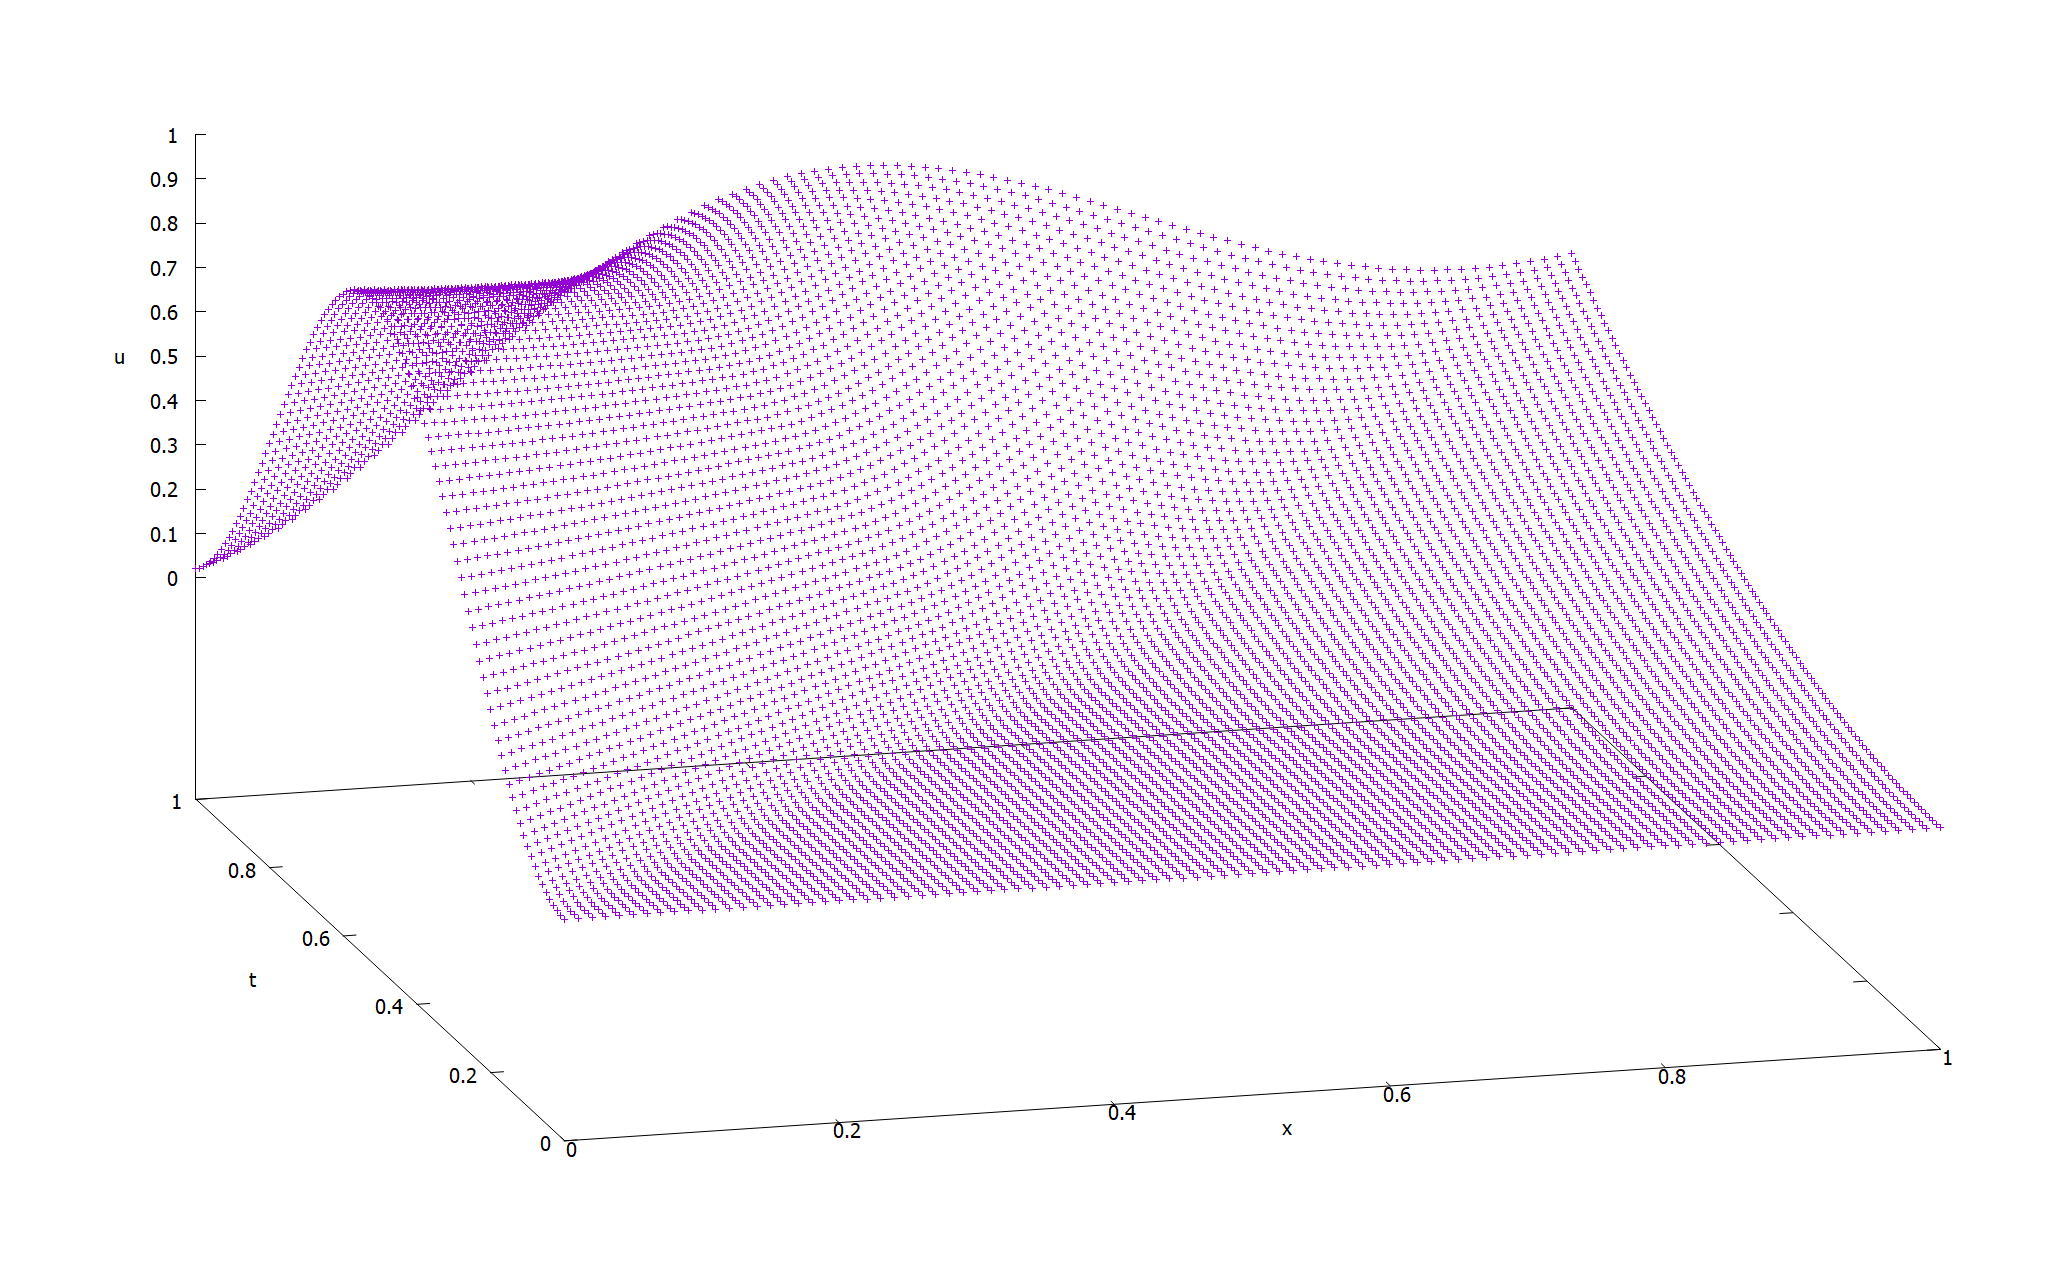
\includegraphics[width=\textwidth]{image_1.png}
		\caption{100 на 100 точек.}
	\end{minipage}
	\hfill
	\begin{minipage}{0.45\textwidth}
		\centering
		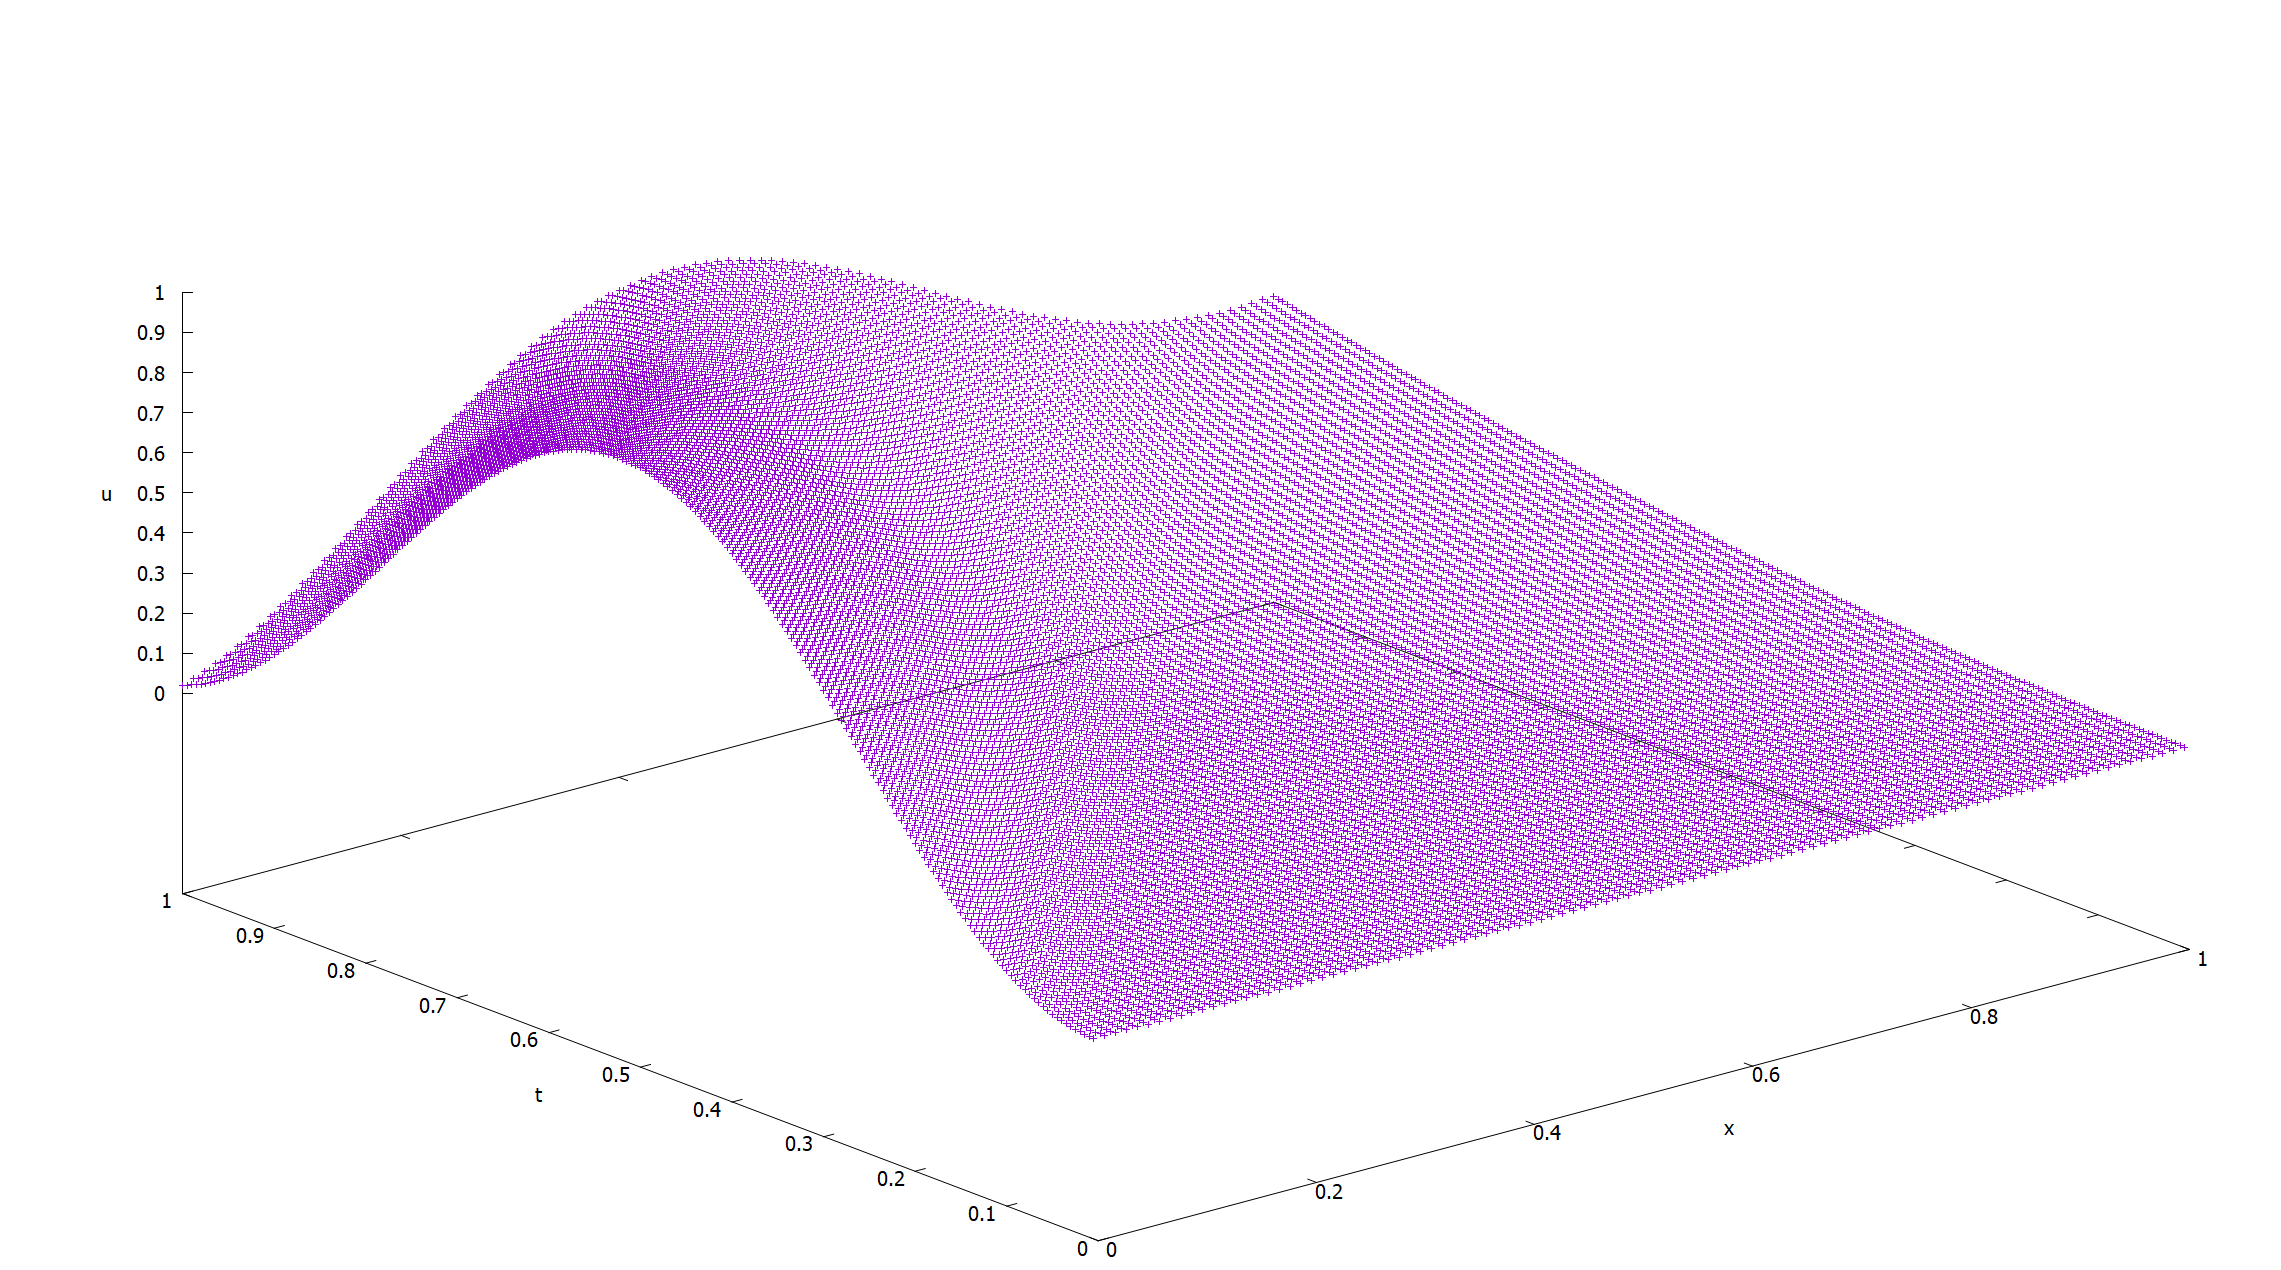
\includegraphics[width=\textwidth]{image_2.png}
		\caption{200 на 100 точек.}
	\end{minipage}
	\hfill
	\newline
	\begin{minipage}{0.45\textwidth}
		\centering
		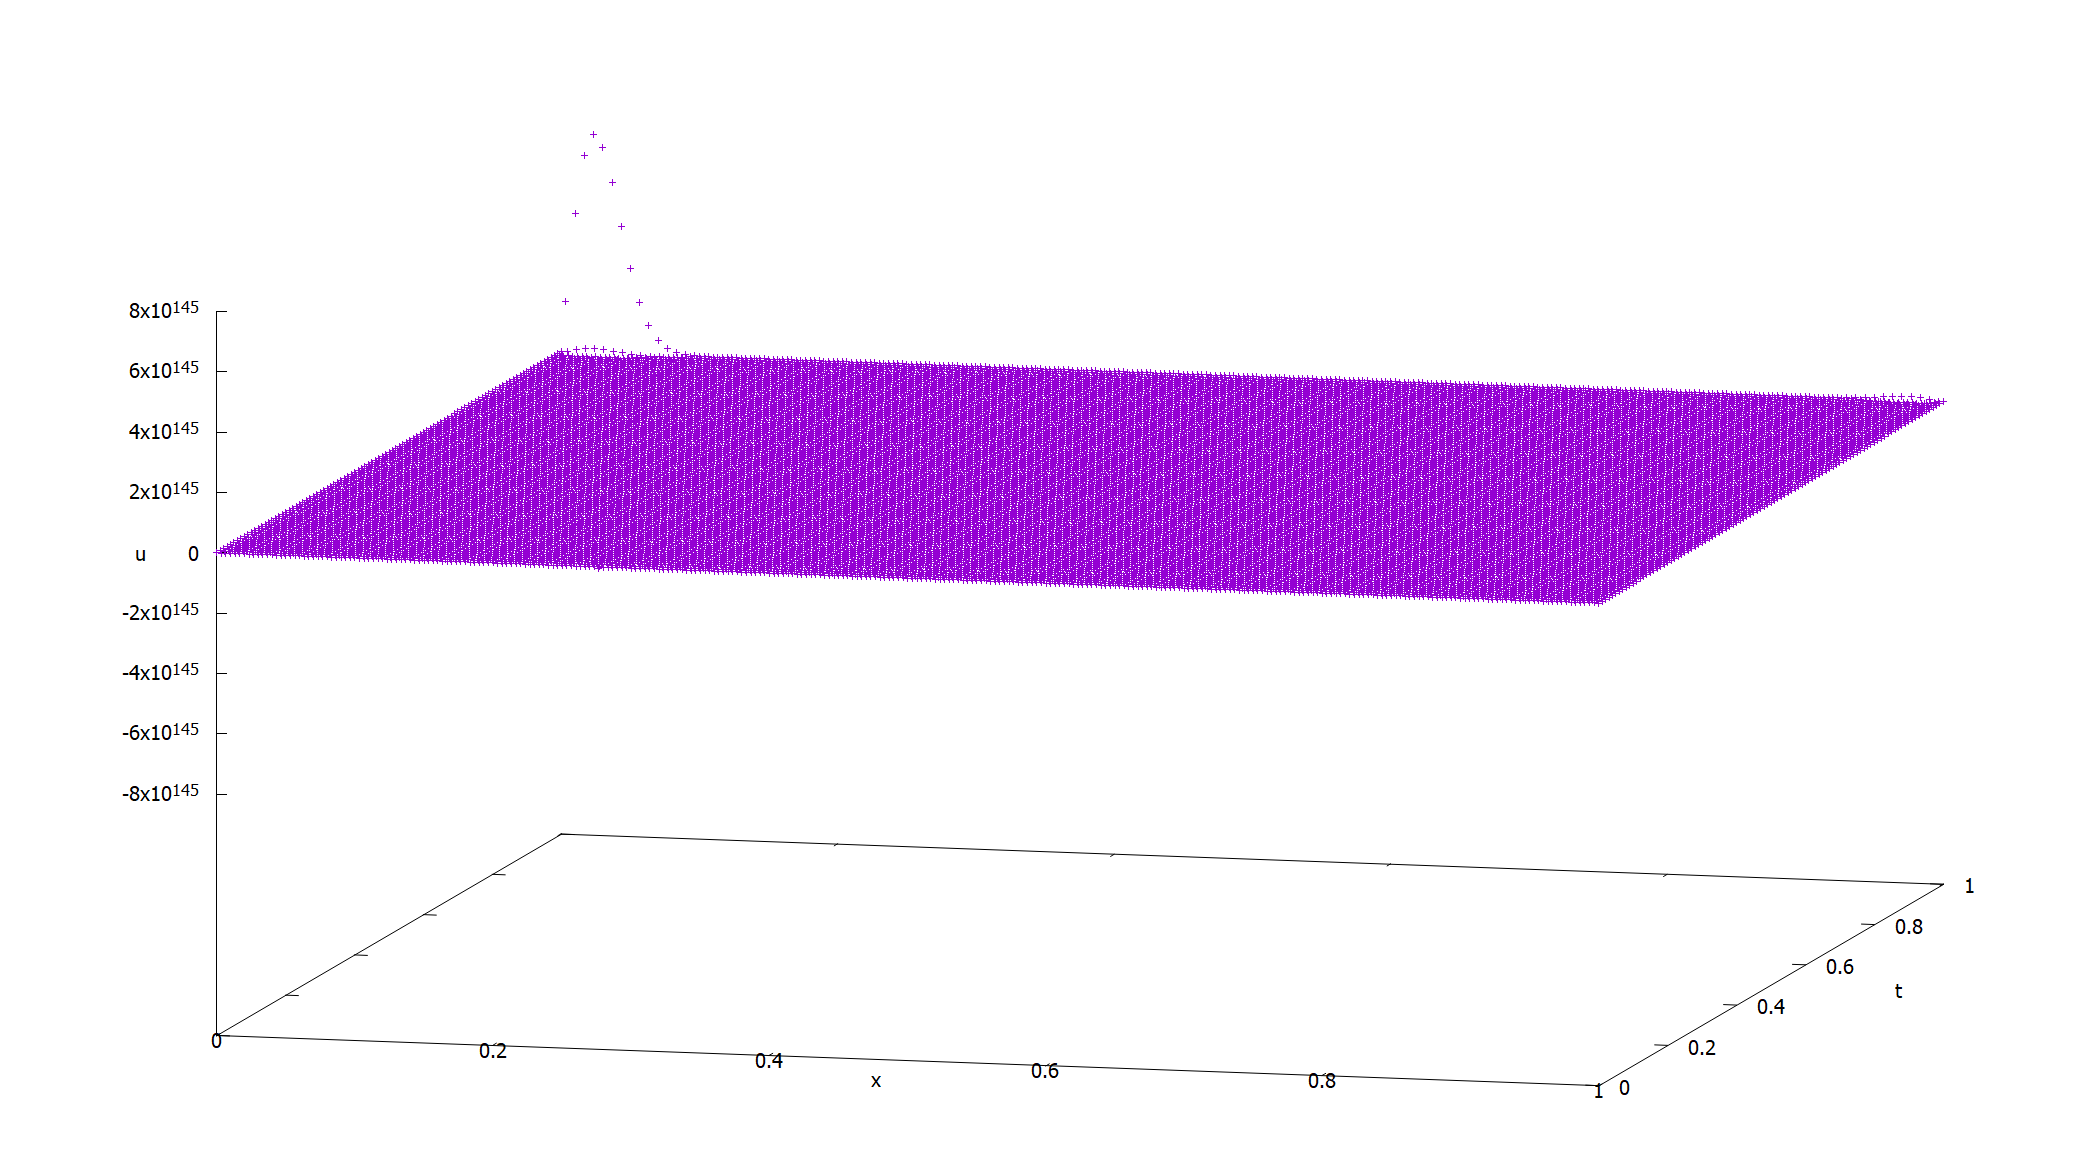
\includegraphics[width=\textwidth]{image_4.png}
		\caption{100 на 200 точек.}
	\end{minipage}
	
	
\end{figure}
	
Из графиков видно, как влияет спектральная устойчивость на решение задачи.
	
	
	
	
	
	
	
	
	
	
	
	
	
	
	
	
	
	
	
	
	
	
	
	
\end{document}
